\documentclass{beamer}

%\useoutertheme[glossy]{wuerzburg}
\useinnertheme[shadow,outline]{chamfered}
%\usecolortheme{shark}
\usecolortheme{beaver}
\beamertemplatenavigationsymbolsempty

\usefonttheme{professionalfonts}
\let\digamma\relax
\usepackage[scale=0.85,stdmathitalics=true,romanfamily=casual]{lucimatx}
\usefonttheme[stillsansseriftext]{serif}



\usepackage{fancyvrb}

%% Fancy syntax coloring via pygments
\usepackage{minted}
\definecolor{bg}{rgb}{0.95,0.95,0.95}
\usemintedstyle{borland}


\newenvironment{Rcode}
{\VerbatimEnvironment
 \begin{minted}[fontsize=\scriptsize,baselinestretch=1]{r}}%
{\end{minted}}

\newenvironment{Pcode}
{\VerbatimEnvironment
 \begin{minted}[fontsize=\scriptsize,baselinestretch=1]{python}}%
{\end{minted}}

\newenvironment{Code}[1]
{\VerbatimEnvironment
 \begin{minted}[fontsize=\scriptsize,baselinestretch=1]{#1}}%
{\end{minted}}


\usepackage{textfit} % commands \scaletoheight{height}{text} and \scaletowidth{width}{text}

\usepackage{tikz}

\usepackage{tcolorbox}

\newtheorem{Alert}{Alert}
\newtheorem{Highlight}{Highlight}

\newcommand{\Species}[1]{{\rmfamily \itshape #1}}
\newcommand{\Real}{\ensuremath{\mathbb{R}}}
\newcommand{\RealN}{\ensuremath{\mathbb{R}^n}}
\newcommand{\RealP}{\ensuremath{\mathbb{R}^p}}
\newcommand{\Mtx}[1]{\ensuremath{\mathbf{#1}}}
\newcommand{\Inv}[1]{\ensuremath{#1^{-1}}}
\newcommand{\InvMtx}[1]{\ensuremath{\mathbf{#1}^{-1}}}
\newcommand{\Red}[1]{\textcolor{red}{#1}}
\newcommand{\PsInv}[1]{\ensuremath{\mathbf{#1}^{+}}}

\usepackage{booktabs}



% --- Macro \xvec
% From a tex.stackexchange.com answer by Todd Lehman
% http://tex.stackexchange.com/questions/44017/dot-notation-for-derivative-of-a-vector
\makeatletter
\newlength\xvec@height%
\newlength\xvec@depth%
\newlength\xvec@width%
\newcommand{\xvec}[2][]{%
  \ifmmode%
    \settoheight{\xvec@height}{$#2$}%
    \settodepth{\xvec@depth}{$#2$}%
    \settowidth{\xvec@width}{$#2$}%
  \else%
    \settoheight{\xvec@height}{#2}%
    \settodepth{\xvec@depth}{#2}%
    \settowidth{\xvec@width}{#2}%
  \fi%
  \def\xvec@arg{#1}%
  \def\xvec@dd{:}%
  \def\xvec@d{.}%
  \raisebox{.2ex}{\raisebox{\xvec@height}{\rlap{%
    \kern.05em%  (Because left edge of drawing is at .05em)
    \begin{tikzpicture}[scale=1]
    \pgfsetroundcap
    \draw (.05em,0)--(\xvec@width-.05em,0);
    \draw (\xvec@width-.05em,0)--(\xvec@width-.15em, .075em);
    \draw (\xvec@width-.05em,0)--(\xvec@width-.15em,-.075em);
    \ifx\xvec@arg\xvec@d%
      \fill(\xvec@width*.45,.5ex) circle (.5pt);%
    \else\ifx\xvec@arg\xvec@dd%
      \fill(\xvec@width*.30,.5ex) circle (.5pt);%
      \fill(\xvec@width*.65,.5ex) circle (.5pt);%
    \fi\fi%
    \end{tikzpicture}%
  }}}%
  #2%
}
\makeatother

% --- Override \vec with an invocation of \xvec.
\let\stdvec\vec
\renewcommand{\vec}[1]{\xvec[]{#1}}
% --- Define \dvec and \ddvec for dotted and double-dotted vectors.
\newcommand{\dvec}[1]{\xvec[.]{#1}}
\newcommand{\ddvec}[1]{\xvec[:]{#1}}


\usepackage{pifont}
\newcommand{\weblink}{\ding{43}}  % hand with pointing finger

\definecolor{links}{HTML}{2A1B81}
\hypersetup{colorlinks,linkcolor=,urlcolor=magenta}

%===========================================================
% Title Info
\title{Scientific Computing for Biologists}
\subtitle{Data as Vectors} % (optional)

\author[P. Magwene]{Instructor: Paul M. Magwene}

\date{04 September 2012}

\begin{document}
%===========================================================
\begin{frame}
\titlepage
\end{frame}

%===========================================================
\begin{frame}
  \frametitle{Overview of Lecture}

\begin{itemize}
		\item Vector Geometry
		\begin{itemize}
			\item Vectors are directed line segments
			\item Vector length
		\end{itemize}
		\item Vector Arithmetic
		\begin{itemize}
			\item Addition, subtraction
			\item Scalar multiplication
			\item Linear combinations of vectors
			\item Dot product and projection
		\end{itemize}
		\item Vector representations of multivariate data
		\begin{itemize}
		  \item Variable space/Subject space representations
			\item Mean as projection in subject space
			\item Bivariate regression in geometric terms
			\item Difference in group means as a regression problem
		\end{itemize}
\end{itemize}

\end{frame}
%===========================================================

%===========================================================
\begin{frame}
  \frametitle{Hands-on Session}
		\begin{itemize}
		  \item Vector operations in R
		  \item Writing functions in R
		  \item Visualizing bivariate relationships in R
		  \item Linear regression in R
	 \end{itemize}
\end{frame}
%===========================================================

%===========================================================
\begin{frame}
  \frametitle{Vector Geometry}

Vectors are directed line segments.

\begin{center}

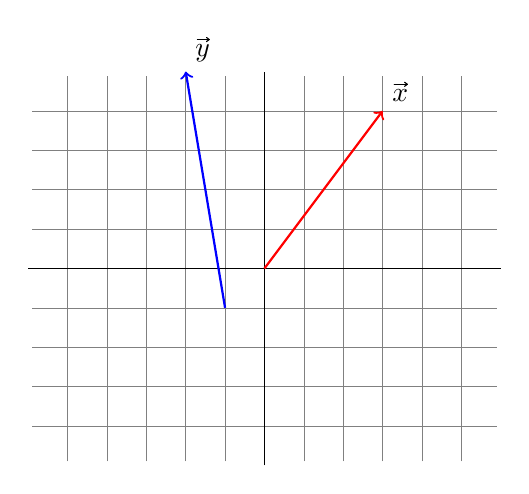
\begin{tikzpicture}[x=0.5cm, y=0.5cm]
\draw[step=0.5cm, style=help lines] (-5.9,-4.9) grid (5.9,4.9);

\draw (-6,0) -- (6,0);
\draw (0,-5) -- (0,5);

\draw[thick,red,->] (0,0) -- (3,4);
\draw (3,4) node[above right] {$\vec{x}$};

\draw[thick,blue,->] (-1,-1) -- (-2,5);
\draw (-2,5) node[above right] {$\vec{y}$};

\end{tikzpicture}

\end{center}

All of the figures and algebraic formulas I show you apply to $n$-dimensional vectors.


\end{frame}
%===========================================================

%===========================================================
\begin{frame}
  \frametitle{Vector Geometry}

Vectors have direction and length:
\[
\vec{x} = [x_1,x_2]' = [2,3]';\; |\vec{x}| = \sqrt{x_1^2 + x_2^2 + \cdots + x_n^2}
\]

\begin{center}

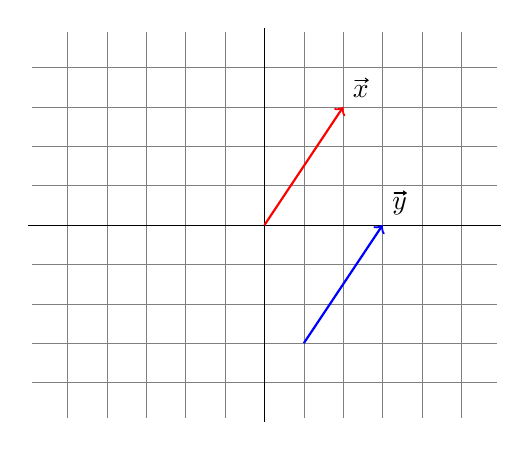
\begin{tikzpicture}[x=0.5cm, y=0.5cm]

\draw[step=0.5cm, style=help lines] (-5.9,-4.9) grid (5.9,4.9);
\draw (-6,0) -- (6,0);
\draw (0,-5) -- (0,5);

\draw[thick,red,->] (0,0) -- (2,3);
\draw (2,3) node[above right] {$\vec{x}$};

\draw[thick,blue,->] (1,-3) -- (3,0);
\draw (3,0) node[above right] {$\vec{y}$};

\end{tikzpicture}
\end{center}

Often starting point is ignored, in which case $\vec{x} = \vec{y}$.


\end{frame}
%===========================================================

%===========================================================
\begin{frame}
  \frametitle{Scalar Multiplication of a Vector}

Let $k$ be a scalar.

\[
k \vec{x} = \left[ \begin{array}{c} k x_1 \\
																		k x_2 \\
																		\vdots \\
																		k x_n \\
\end{array} \right]
\]

\begin{center}

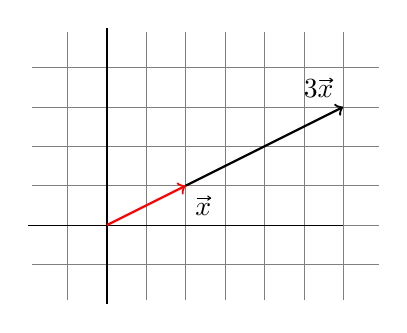
\begin{tikzpicture}[x=0.5cm, y=0.5cm]

\draw[step=0.5cm, style=help lines] (-1.9,-1.9) grid (6.9,4.9);
\draw (-2,0) -- (6,0);
\draw (0,-2) -- (0,5);

\draw[thick,red,->] (0,0) -- (2,1);
\draw (2,1) node[below right] {$\vec{x}$};

\draw[thick,->] (2,1) -- (6,3);
\draw (6,3) node[above left] {$3 \vec{x}$};

\end{tikzpicture}

$\vec{x} = [2,1]'; \; 3\vec{x} = [6,3]'$.

\end{center}




\end{frame}
%===========================================================

%===========================================================
\begin{frame}
  \frametitle{Vector Addition}

Let $\vec{x} = [2,1]'; \; \vec{y} = [1,3]'$

\[
\vec{z} = \vec{x} + \vec{y} = \left[ \begin{array}{c} x_1 + y_1 \\
															x_2 + y_2 \\
															\vdots \\
															x_n + y_n
\end{array} \right]
\]

\begin{center}

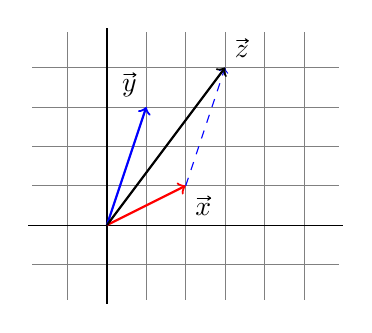
\begin{tikzpicture}[x=0.5cm, y=0.5cm]

\draw[step=0.5cm, style=help lines] (-1.9,-1.9) grid (5.9,4.9);
\draw (-2,0) -- (6,0);
\draw (0,-2) -- (0,5);

\draw[thick,red,->] (0,0) -- (2,1);
\draw (2,1) node[below right] {$\vec{x}$};

\draw[thin,blue,dashed,->] (2,1) -- ++(1,3);

\draw[thick,blue,->] (0,0) -- (1,3);
\draw (1,3) node[above left] {$\vec{y}$};


\draw[thick,->] (0,0) -- (3,4);
\draw (3,4) node[above right] {$\vec{z}$};

\end{tikzpicture}
\end{center}

Addition follows the `head-to-tail' rule.


\end{frame}
%===========================================================

%===========================================================
\begin{frame}
  \frametitle{Vector Subtraction}

Let $\vec{x} = [2,1]'; \; \vec{y} = [1,3]'$

\[
\vec{z} = \vec{x} - \vec{y} = \left[ \begin{array}{c} x_1 - y_1 \\ x_2 - y_2 \end{array} \right] =
															\left[ \begin{array}{c} 1 \\ -2 \end{array} \right]
\]

\begin{center}

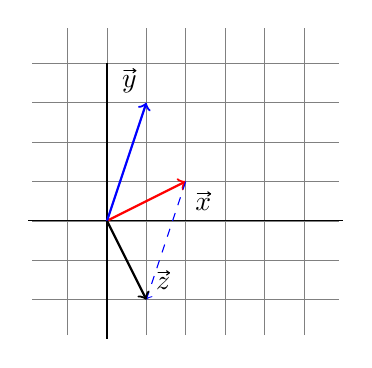
\begin{tikzpicture}[x=0.5cm, y=0.5cm]

\draw[step=0.5cm, style=help lines] (-1.9,-2.9) grid (5.9,4.9);
\draw (-2,0) -- (6,0);
\draw (0,-3) -- (0,4);

\draw[thick,red,->] (0,0) -- (2,1);
\draw (2,1) node[below right] {$\vec{x}$};

\draw[thin,blue,dashed,->] (2,1) -- ++(-1,-3);

\draw[thick,blue,->] (0,0) -- (1,3);
\draw (1,3) node[above left] {$\vec{y}$};


\draw[thick,->] (0,0) -- (1,-2);
\draw (1,-2) node[above right] {$\vec{z}$};

\end{tikzpicture}
\end{center}

Follow the addition rule for $-1 \vec{y}$.


\end{frame}
%===========================================================

%===========================================================
\begin{frame}
  \frametitle{Linear Combinations of Vectors}

A linear combination of vectors is of the form $z = b_1 \vec{x} + b_2 \vec{y}$


\[
\vec{z} = 3\vec{x} - 0.5\vec{y} = 3 \left[ \begin{array}{c} x_1  \\ x_2  \end{array} \right] -
															0.5 \left[ \begin{array}{c} y_1 \\ y_2 \end{array} \right]
\]

\begin{center}

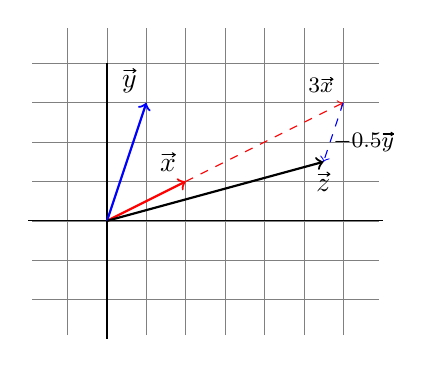
\begin{tikzpicture}[x=0.5cm, y=0.5cm]

\draw[step=0.5cm, style=help lines] (-1.9,-2.9) grid (6.9,4.9);
\draw (-2,0) -- (7,0);
\draw (0,-3) -- (0,4);

\draw[thick,red,->] (0,0) -- (2,1);
\draw (2,1) node[above left] {$\vec{x}$};

\draw[thin,red,dashed,->] (2,1) -- (6,3);
\draw (6,3) node[above left,font=\footnotesize] {$3\vec{x}$};

\draw[thin,blue,dashed,->] (6,3) -- (5.5,1.5);
\draw (5.5, 1.5) node[above right, font=\footnotesize] {$-0.5\vec{y}$};

\draw[thick,blue,->] (0,0) -- (1,3);
\draw (1,3) node[above left] {$\vec{y}$};

\draw[thick,->] (0,0) -- (5.5, 1.5);
\draw (5.5, 1.5) node[below] {$\vec{z}$};

\end{tikzpicture}
\end{center}


\end{frame}
%===========================================================

%===========================================================
\begin{frame}
  \frametitle{Dot Product}

The dot (inner) product of two vectors, $\vec{x} \cdot \vec{y}$ is a scalar.
%
\begin{eqnarray*}
\vec{x} \cdot \vec{y}  & = & x_1 y_1 + x_2 y_2 + \cdots + x_n y_n \\
								      & = & |\vec{x}||\vec{y}| \cos \theta
\end{eqnarray*}
%
where $\theta$ is the angle (in radians) between $\vec{x}$ and $\vec{y}$

\begin{center}

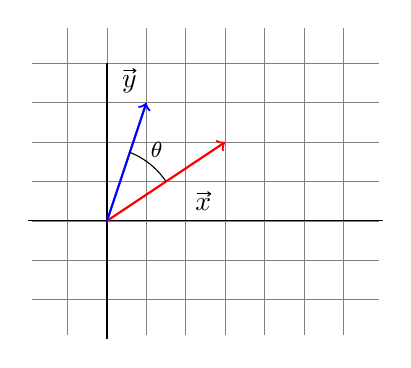
\begin{tikzpicture}[x=0.5cm, y=0.5cm]

\draw[step=0.5cm, style=help lines] (-1.9,-2.9) grid (6.9,4.9);
\draw (-2,0) -- (7,0);
\draw (0,-3) -- (0,4);

\draw[thick,red,->] (0,0) -- (3,2);
\draw (2,1) node[below right] {$\vec{x}$};

\draw[thick,blue,->] (0,0) -- (1,3);
\draw (1,3) node[above left] {$\vec{y}$};

\draw (1.5,1) arc (34:69:1cm);
\path (0,0) ++(55:1.1cm) node[font=\footnotesize] {$\theta$};

\end{tikzpicture}

$ \vec{x} = [3,2]', \vec{y} = [1,3]'; \; \vec{x} \cdot \vec{y} = \sqrt{13}\sqrt{10}\cos \theta = 9$

\end{center}


\end{frame}
%===========================================================

%===========================================================
\begin{frame}
  \frametitle{Useful Geometric Quantities as Dot Product}


Length:
\begin{eqnarray*}
|\vec{x}|^2 & = & \vec{x} \cdot \vec{x}  =  x_1^2 + x_2^2 + \cdots + x_n^2\\
|\vec{y}|^2 & = & \vec{y} \cdot \vec{y}
\end{eqnarray*}

Distance:
\begin{eqnarray*}
|\vec{x}-\vec{y}|^2 = \vec{x} \cdot \vec{x} + \vec{y} \cdot \vec{y} - 2 \vec{x} \cdot \vec{y}
\end{eqnarray*}

Angle:
\begin{eqnarray*}
\cos \theta = \vec{x} \cdot \vec{y}/(|x||y|)
\end{eqnarray*}

\begin{center}

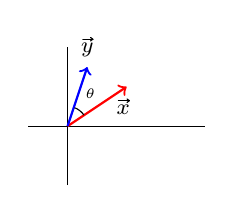
\begin{tikzpicture}[x=0.25cm, y=0.25cm]

\draw (-2,0) -- (7,0);
\draw (0,-3) -- (0,4);

\draw[thick,red,->] (0,0) -- (3,2);
\draw (2,1) node[right,font=\footnotesize] {$\vec{x}$};

\draw[thick,blue,->] (0,0) -- (1,3);
\draw (1,3) node[above,,font=\footnotesize] {$\vec{y}$};

\draw (0,0) +(34:0.25cm) arc (34:69:0.25cm);
\path (0,0) ++(55:0.5cm) node[font=\tiny] {$\theta$};

\end{tikzpicture}

\end{center}

\end{frame}
%===========================================================

%===========================================================
\begin{frame}
  \frametitle{Dot Product Properties}

Some additional properties of the dot product that are useful to know:

\begin{eqnarray*}
\vec{x} \cdot \vec{y} & = & \vec{y} \cdot \vec{x} \ \mbox{(commutative)} \\
\vec{x} \cdot (\vec{y} + \vec{z}) & = & \vec{x} \cdot \vec{y} + \vec{x} \cdot \vec{z} \ \mbox{(distributive)}\\
(k\vec{x}) \cdot \vec{y} & = & \vec{x} \cdot (k\vec{y}) = k(\vec{x} \cdot \vec{y}) \ \mbox{where $k$ is a scalar} \\
\vec{x} \cdot \vec{y} & = & 0 \ \mbox{iff $\vec{x}$ and $\vec{y}$ are orthogonal}
\end{eqnarray*}

\end{frame}
%===========================================================


%===========================================================
\begin{frame}
  \frametitle{Vector Projection}

The projection of $\vec{y}$ onto $\vec{x}$, $P_{\vec{x}}(\vec{y})$, is the vector obtained by placing $\vec{y}$ and $\vec{x}$ tail to tail and dropping a line, perpendicular to $\vec{x}$, from the head of $\vec{y}$ onto the line defined by $\vec{x}$.
\[
P_{\vec{x}}(\vec{y}) = \left(\frac{\vec{x} \cdot \vec{y}}{|\vec{x}|}\right) \frac{\vec{x}}{|\vec{x}|} = \left(\frac{\vec{x} \cdot \vec{y}}{|\vec{x}|^2}\right)\vec{x}
\]

The component of $\vec{y}$ in $\vec{x}$, $C_{\vec{x}}(\vec{y})$, is the length of $P_{\vec{x}}(\vec{y})$.
\[
C_{\vec{x}}(\vec{y}) = \frac{\vec{x} \cdot \vec{y}}{|\vec{x}|} = |\vec{y}|\cos \theta
\]

\begin{center}

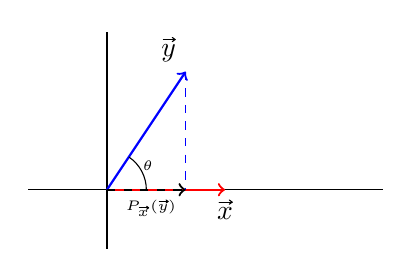
\begin{tikzpicture}[x=0.5cm, y=0.5cm]

\draw (-2,0) -- (7,0);
\draw (0,-1.5) -- (0,4);

\draw[thick,red,->] (0,0) -- (3,0);
\draw (3,0) node[below] {$\vec{x}$};

\draw[thick,blue,->] (0,0) -- (2,3);
\draw (2,3) node[above left] {$\vec{y}$};

\draw[thin,blue,dashed] (2,3) -- (2,0);

\draw[thick, dashed,->] (0,0) -- (2,0);
\draw (2,0) node[below left,font=\tiny] {$P_{\vec{x}}(\vec{y})$};

\draw (0,0) +(0:0.5cm) arc (0:56:0.5cm);
\path (0,0) ++(30:0.6cm) node[font=\tiny] {$\theta$};


\end{tikzpicture}


\end{center}


\end{frame}
%===========================================================

%===========================================================
\begin{frame}
  \frametitle{Vector Projection II}

$\vec{y}$ can be decomposed into a a vector parallel to $\vec{x}$, $\widehat{y} = P_{\vec{x}}(\vec{y})$, and a vector perpendicular to $\vec{x}$, $\widehat{y}_{\bot}$.

\[
\vec{y} = \widehat{y} + \widehat{y}_{\bot}
\]

\begin{center}

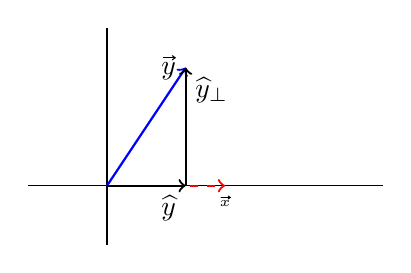
\begin{tikzpicture}[x=0.5cm, y=0.5cm]

\draw (-2,0) -- (7,0);
\draw (0,-1.5) -- (0,4);

\draw[thick,red,dashed,->] (0,0) -- (3,0);
\draw (3,0) node[below,font=\tiny] {$\vec{x}$};

\draw[thick,blue,->] (0,0) -- (2,3);
\draw (2,3) node[left] {$\vec{y}$};

\draw[thick, ->] (2,0) -- (2,3);
\draw (2,3) node[below right] {$\widehat{y}_{\bot}$};

\draw[thick,->] (0,0) -- (2,0);
\draw (2,0) node[below left] {$\widehat{y}$};

\end{tikzpicture}
\end{center}

\begin{itemize}
 \item $\widehat{y}_{\bot}$ is \emph{orthogonal} to $\widehat{y}$ and $\vec{x}$.
 \item $\widehat{y}$  is the closest vector to $\vec{y}$ in the subspace defined by $\vec{x}$
\end{itemize}

\end{frame}
%===========================================================

%===========================================================
\begin{frame}

\begin{center}
\LARGE{Vector Geometry of Simple Statistics}
\end{center}


\end{frame}
%===========================================================


%===========================================================
\begin{frame}
  \frametitle{Variable Space Representation of a Data Set}

Consider a data set in which we've measured variables $\mathbf{X} = {X_1, X_2,\ldots,X_p}$, on a set of subjects (objects) $a_1,...,a_n$.

\begin{center}
	\begin{tabular}{l|cc}

 & $X_1$ & $X_2$ \\ \hline

$a_1$ & 0.9 & 1.4 \\
$a_2$ & 1.1 & 1.7 \\
$\vdots$ & $\vdots$ & $\vdots$ \\
$a_n$ & 0.5 &  1.55

	\end{tabular}
\end{center}

Such data is most often represented by drawing the objects as points in space of dimension $p$. This is the \emph{variable space representation} of the data.

\begin{center}

\begin{tikzpicture}[x=0.25cm, y=0.25cm]

\draw[->] (-8,0) -- (8,0);
\draw (8,0) node[right,font=\footnotesize] {$X_1$};

\draw[->] (0,-4) -- (0,4);
\draw (0,4) node[above,font=\footnotesize] {$X_2$};

\draw plot[only marks, mark=ball] coordinates { (-3.5,-1) (-3,-2) (-1,-1.5) (-1,0.25) (0,-1.5) (0,0.1) (0.5,1.6) (1,2.5) (2,0.5) (2,3) (3,2.5) };

\end{tikzpicture}
\end{center}


\end{frame}
%===========================================================

%===========================================================
\begin{frame}
  \frametitle{Subject Space Representation of a Data Set}

\begin{small}

An alternate representation is to consider the variables in the space of the subjects. This is the \emph{subject space} representation.
\begin{itemize}
\item trickier to visualize because high dimensional
\end{itemize}

How then do we come up with a useful representation of variables in subject space?
\begin{itemize}
 \item Any pair of non-parallel vectors (of arbitrary dimension) defines a plane.
 \item Let the variables be represented by centered vectors
 \begin{itemize}
    \item lengths of vectors are proportional to standard deviation
 	\item angle between vectors represents association or similarity
 \end{itemize}
\end{itemize}
\end{small}

\begin{center}

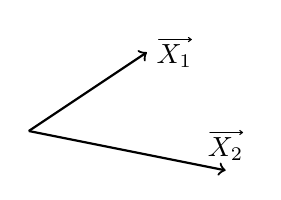
\begin{tikzpicture}[x=0.5cm, y=0.5cm]

\draw[thick,->] (0,0) -- (3,2);
\draw (3,2) node[right] {$\vec{X_1}$};

\draw[thick,->] (0,0) -- (5,-1);
\draw (5,-1) node[above] {$\vec{X_2}$};

\end{tikzpicture}
\end{center}


\end{frame}
%===========================================================

%===========================================================
\begin{frame}
  \frametitle{Geometry of the Mean in Subject Space}

The mean, as you know, is the `optimal' (in a least square sense) single number summary of a variable of interest.

\begin{itemize}

\item The mean, $\bar{x}$, minimizes the quantity $\sum_{i=1}^{n}(x_i-\bar{x})^2$.

\item The above can be written as $|\vec{\mathbf{x}}-\vec{\mathbf{1}}\bar{x}|^2$ where $\vec{\mathbf{1}} = [1,1,\ldots,1]'$

\item We are looking, therefore, for the scalar multiple, $\bar{x}$, of the unit vector that minimizes $|\vec{\mathbf{x}}-\vec{\mathbf{1}}\bar{x}|^2$

\end{itemize}
\end{frame}
%===========================================================

%===========================================================
\begin{frame}
  \frametitle{Geometry of the Mean in Subject Space II}

Geometric derivation of the sample mean:

\begin{center}

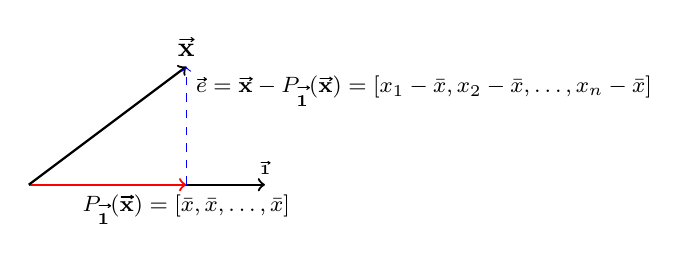
\begin{tikzpicture}[x=0.5cm, y=0.5cm]

\draw[thick,->] (0,0) -- (6,0);
\draw (6,0) node[above,font=\tiny] {$\vec{\mathbf{1}} $};

\draw[thick,red,->] (0,0) -- (4,0);
\draw (4,0) node[below,font=\footnotesize] {$P_{\vec{\mathbf{1}}}(\vec{\mathbf{x}}) = [\bar{x}, \bar{x},\ldots,\bar{x}]$};

\draw[thick,->] (0,0) -- (4,3);
\draw (4,3) node[above] {$\vec{\mathbf{x}}$};

\draw[dashed,blue,->] (4,0) -- (4,3);
\draw (4,3) node[below right,font=\footnotesize] {$\vec{e} = \vec{\mathbf{x}} - P_{\vec{\mathbf{1}}}(\vec{\mathbf{x}}) = [x_1-\bar{x}, x_2 - \bar{x},\ldots,x_n - \bar{x}]$};

\end{tikzpicture}
\end{center}


\end{frame}
%===========================================================

%===========================================================
\begin{frame}
  \frametitle{Geometry of the Mean in Subject Space III}

\begin{itemize}
\item Recall that:
\begin{eqnarray}
P_{\vec{\mathbf{1}}}(\vec{\mathbf{x}}) & = & \vec{\mathbf{1}}\bar{x} \ \mbox{for some}\ \bar{x} \\
%
(\vec{\mathbf{x}} - P_{\vec{\mathbf{1}}}(\vec{\mathbf{x}})) \cdot \vec{\mathbf{1}} & = & 0
\end{eqnarray}

\item Substituting (1) into (2):
\begin{eqnarray}
(\vec{\mathbf{x}} - \vec{\mathbf{1}}\bar{x}) \cdot \vec{\mathbf{1}} & = & 0 \\
%
\vec{\mathbf{x}} \cdot \vec{\mathbf{1}} & = & \bar{x} (\vec{\mathbf{1}} \cdot \vec{\mathbf{1}})
\end{eqnarray}

\item Expanding (4):
\begin{eqnarray}
x_1 + x_2 + \cdots + x_n & = & n \bar{x} \\
%
\sum x_i & = & n \bar{x} \\
%
\bar{x} & = & (1/n) \sum x_i
\end{eqnarray}

\end{itemize}


\end{frame}
%===========================================================



%===========================================================
\begin{frame}[shrink]
  \frametitle{Geometry of Sample Variance}

\begin{itemize}

\item $|\vec{e}|^2$ is the sum of squared errors (SSE).

\item What is the dimensionality of $\vec{e}$?

\begin{itemize}
	\item Because $\vec{e}$ is orthogonal to the $n$-dimensional unit vector $\vec{\mathbf{1}}$, it must lie in a subpace of dimensionality $n-1$.
\end{itemize}

\item The mean squared error (MSE) is the average error `per dimension'
\begin{eqnarray*}
MSE & = & |\vec{e}|^2/(n-1) \\
     & =& \frac{1}{(n-1)} \sum (x_i - \bar{x})^2 \leftarrow \ \mbox{\textbf{Sample Variance!}}
\end{eqnarray*}

\end{itemize}
\begin{center}
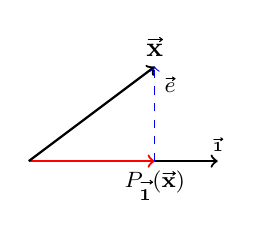
\begin{tikzpicture}[x=0.4cm, y=0.4cm]

\draw[thick,->] (0,0) -- (6,0);
\draw (6,0) node[above,font=\tiny] {$\vec{\mathbf{1}} $};

\draw[thick,red,->] (0,0) -- (4,0);
\draw (4,0) node[below,font=\footnotesize] {$P_{\vec{\mathbf{1}}}(\vec{\mathbf{x}})$};

\draw[thick,->] (0,0) -- (4,3);
\draw (4,3) node[above] {$\vec{\mathbf{x}}$};

\draw[dashed,blue,->] (4,0) -- (4,3);
\draw (4,3) node[below right,font=\footnotesize] {$\vec{e}$};

\end{tikzpicture}
\end{center}
This is a nice geometric demonstration of why the degrees of freedom of the sample variance is $n-1$.


\end{frame}
%===========================================================

%===========================================================
\begin{frame}
  \frametitle{Correlation in Vector Geometric Terms}

Let $X$ and $Y$ be mean centered variables, and let $\vec{x}$ and $\vec{y}$ be their corresponding vector representations in subject space.

\begin{center}

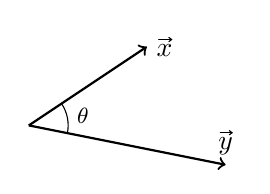
\begin{tikzpicture}[x=0.5cm, y=0.5cm]

\draw[thick,->] (0,0) -- (3,2);
\draw (3,2) node[right] {$\vec{x}$};

\draw[thick,->] (0,0) -- (5,-1);
\draw (5,-1) node[above] {$\vec{y}$};

\draw (0,0) +(-11:0.5cm) arc (-11:34:0.5cm);
\path (0,0) ++(10:0.7cm) node[font=\footnotesize] {$\theta$};

\end{tikzpicture}
\end{center}

\[
\mathsf{cor}(X,Y) = r_{XY} = \cos \theta = \frac{\vec{x} \cdot \vec{y}}{|\vec{x}||\vec{y}|}
\]


\end{frame}
%===========================================================


%===========================================================
\begin{frame}
  \frametitle{Bivariate Regression as Projection}

The standard bivariate regression equation relating one observed variable $X$ (the predictor) to another observed variable of interest, $Y$ (the outcome) is usually written as:
\[
\widehat{Y} = a + bX.
\]
where $\widehat{Y}$ is the predicted value of $Y$ and $a$ and $b$ are scalar values chosen to minimize $|Y-\widehat{Y}|$.

\medskip

Let's express this in vector terms, and work with mean-centered vectors so the equation becomes:
\[
\vec{\widehat{y}} = b\vec{x}
\]
See Wickens Chapt 3 for the general derivation for uncentered variables.

\end{frame}
%===========================================================

%===========================================================
\begin{frame}[allowframebreaks]
  \frametitle{Derivation: Bivariate Regression as Projection}

Regression equation for mean-centered vectors: $\vec{\widehat{y}} = b\vec{x}$

\begin{itemize}
\item Our goal is to choose the scalar $b$ such that the error vector $\vec{e} = \vec{y} - \vec{\widehat{y}}$ is as small as possible.

\item We've already seen this problem when we derived the mean. We're trying to solve for $b$ in the equation:
%
\begin{eqnarray*}
(\vec{y} - b\vec{x}) \cdot \vec{x} &=& 0 \\
\vec{x} \cdot \vec{y} &=& b(\vec{x} \cdot \vec{x})
\end{eqnarray*}

\item Solving for $b$ we get:
%
\[
b = \frac{\vec{x} \cdot \vec{y}}{(\vec{x} \cdot \vec{x})} = \frac{\vec{x} \cdot \vec{y}}{|\vec{x}|^2}
\]

\item We can also rewrite $b = (\vec{x} \cdot \vec{y})/|\vec{x}|^2$ as
%
%\begin{eqnarray*}
\[
b = \frac{|x||y| \cos \theta}{|x|^2}
  = \cos \theta \frac{|y|}{|x|}
  = r_{XY} \frac{|y|}{|x|}
\]
%\end{eqnarray*}

\end{itemize}


\end{frame}
%===========================================================

%===========================================================
\begin{frame}
  \frametitle{Geometry of Bivariate Regression}

Geometric interpretation of regression as projection:

\begin{center}

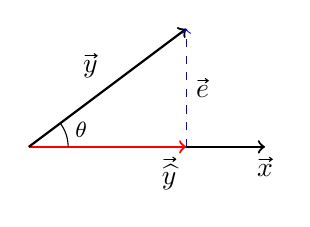
\begin{tikzpicture}[x=0.5cm, y=0.5cm]

\draw[thick,->] (0,0) -- (6,0);
\draw (6,0) node[below] {$\vec{x} $};

\draw[thick,red,->] (0,0) -- (4,0);
\draw (4,0) node[below left] {$\vec{\widehat{y}}$};

\draw[thick,->] (0,0) -- (4,3);
\draw (2,1.5) node[above left] {$\vec{y}$};

\draw[dashed,blue,->] (4,0) -- (4,3);
\draw (4,1.5) node[right] {$\vec{e}$};

\draw (0,0) +(0:0.5cm) arc (0:37:0.5cm);
\path (0,0) ++(18:0.7cm) node[font=\footnotesize] {$\theta$};

\end{tikzpicture}

\[
\vec{\widehat{y}} = b\vec{x}
\]
\begin{eqnarray*}
b &=& |x||y| \cos \theta / |x|^2 \\
  &=& \cos \theta (|y|/|x|) \\
  &=& r_{XY}(|y|/|x|)
\end{eqnarray*}

\end{center}

\end{frame}
%===========================================================


%===========================================================
\begin{frame}
  \frametitle{Bivariate Regression, Goodness of Fit}

How well does our prediction agree with our outcome?

\begin{itemize}
  \item Measure the angle between $\vec{\widehat{y}}$ and $\vec{y}$:
\[
R = \cos \theta_{\vec{y},\vec{\widehat{y}}} = \frac{|\vec{\widehat{y}}|}{|\vec{y}|}
\]

 \item In the single-predictor case $R = r_{XY}$, but this is not generally true when we have multiple predictors.

 \item Note that $|\vec{y}|$ can be expressed as follows:
\begin{eqnarray*}
|\vec{\widehat{y}}|^2 + |\vec{e}|^2 &=& |\vec{y}|^2 \\
SS_\mathit{regression} + SS_\mathit{residual} &=& SS_\mathit{total}
\end{eqnarray*}

 \item With simple substitution we can show that:
\begin{eqnarray*}
SS_\mathit{regression} &=& R^2 SS_\mathit{total} \\
SS_\mathit{residual} &=& (1-R^2)SS_\mathit{total}
\end{eqnarray*}

\end{itemize}


\end{frame}
%===========================================================

%===========================================================
\begin{frame}
  \frametitle{Geometry of Goodness of Fit}

Geometric interpretation of regression goodness-of-fit:

\begin{center}

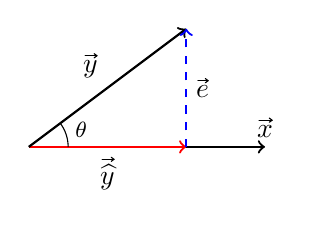
\begin{tikzpicture}[x=0.5cm, y=0.5cm]

\draw[thick,->] (0,0) -- (6,0);
\draw (6,0) node[above] {$\vec{x}$};

\draw[thick,red,->] (0,0) -- (4,0);
\draw (2,0) node[below] {$\vec{\widehat{y}}$};

\draw[thick,->] (0,0) -- (4,3);
\draw (2,1.5) node[above left] {$\vec{y}$};

\draw[thick,dashed,blue,->] (4,0) -- (4,3);
\draw (4,1.5) node[right] {$\vec{e}$};

\draw (0,0) +(0:0.5cm) arc (0:37:0.5cm);
\path (0,0) ++(18:0.7cm) node[font=\footnotesize] {$\theta$};

\end{tikzpicture}

\(
\begin{array}{c}
R = \cos \theta \\
|\vec{\widehat{y}}|^2 + |\vec{e}|^2 = |\vec{y}|^2
\end{array}
\)

\end{center}

\end{frame}
%===========================================================




\end{document}
